\documentclass[runningheads]{llncs}
\usepackage{graphicx}
\usepackage{booktabs}
\usepackage{multirow}
\usepackage{hyperref}
\usepackage{tikz}
\usetikzlibrary{arrows.meta, positioning, shapes.geometric, fit, backgrounds}

\begin{document}

\title{Relict: A Reproducible Open-Source Platform for Environmental DNA Analysis with Integrated Conservation Cross-Referencing}

\author{Shaurya Punj}

\institute{
Thapar Institute of Engineering and Technology, Patiala, Punjab, India \\
\email{workwithshaurya10@gmail.com}
}

\maketitle

\begin{abstract}
Environmental DNA metabarcoding has matured into a widely adopted method for non-invasive biodiversity assessment, yet a persistent disconnect exists between the generation of raw sequencing data and the delivery of ecologically interpretable outputs. Current bioinformatics pipelines handle denoising and taxonomy assignment effectively but leave conservation interpretation, reproducibility documentation, and standardised data submission entirely to the end user. This paper describes Relict, an open-source web platform that integrates a seven-stage amplicon analysis pipeline built on established tools (fastp, vsearch, scikit-bio) with three capabilities absent from existing alternatives: automated per-species conservation status lookup against the Global Biodiversity Information Facility and the IUCN Red List, generation of Darwin Core Archives suitable for citizen-science data publication, and signed provenance manifests that record every input hash, tool version, and pipeline parameter for independent verification. The platform supports six amplicon markers across version-pinned reference databases including SILVA 138.1 and MIDORI2 GenBank 269. Validation against a synthetic known-composition dataset yielded mathematically exact diversity metrics, while processing of a published SRA dataset (ERR2283086, 45,204 reads) produced 51 amplicon sequence variants with complete taxonomy assignment in under four minutes. The software is freely available under the MIT licence.

\keywords{Environmental DNA \and Metabarcoding \and Bioinformatics Pipeline \and Conservation \and Reproducible Research \and GBIF \and IUCN Red List \and Citizen Science}
\end{abstract}

\section{Introduction}

The routine application of environmental DNA sampling for biodiversity surveys has expanded considerably since the foundational work of Ficetola et al.\ on amphibian detection from water samples \cite{ficetola2008}. Organisms continuously release genetic material into their surroundings through mucus, faeces, epidermal cells, and decomposition, and the recovery and sequencing of this material provides a non-invasive alternative to traditional capture-based monitoring \cite{taberlet2012, deiner2017}. The technique has demonstrated particular value for detecting rare and elusive species \cite{pfleger2016}, tracking invasive species spread \cite{larson2020}, and conducting broad-scale community assessments of aquatic and terrestrial ecosystems \cite{bonfil2021}.

The bioinformatics landscape for processing amplicon sequencing data has reached a reasonable level of maturity. Tools such as QIIME~2 \cite{bolyen2019}, DADA2 \cite{callahan2016}, mothur \cite{schloss2011}, and vsearch \cite{rognes2016} each provide reliable implementations of quality control, denoising, clustering, and taxonomic classification. More recent contributions including OBITools \cite{boyer2016} and SimpleMetaPipeline \cite{williams2024} have sought to lower the barrier to entry by wrapping multiple tools into streamlined workflows.

Despite this progress, three functional gaps remain unaddressed by any single existing platform.

First, the step between obtaining a species list and understanding its conservation significance is entirely manual. Researchers who wish to determine whether their detections include threatened, endangered, or invasive species must individually query the IUCN Red List, GBIF occurrence databases, or national protection schedules. This manual process introduces delays and creates opportunities for oversight, particularly in large multi-sample studies \cite{lee2024}.

Second, although workflow management systems such as Snakemake and Nextflow record execution parameters, no eDNA-specific tool generates a self-contained provenance manifest that captures input file checksums, exact software versions, reference database identities, and output hashes in a format ready for inclusion as supplementary material. The absence of such documentation has been identified as a contributing factor to reproducibility challenges in ecological research \cite{powers2019, sandve2013}.

Third, citizen-science organisations and non-specialist monitoring groups increasingly collect eDNA samples but lack the technical infrastructure to convert raw sequencing output into standardised data submissions for global biodiversity databases. The Darwin Core Archive format required by GBIF \cite{gbif2023} involves specific file structures and controlled vocabularies that remain inaccessible without dedicated tooling.

This paper presents Relict, an integrated platform that addresses all three gaps within a single deployable system. The platform combines a containerised bioinformatics pipeline with a web-based interface, automated conservation cross-referencing, provenance manifest generation, and one-click export to GBIF-compatible formats.

\section{Design Rationale}

The development of Relict was guided by eight engineering principles selected to address observed shortcomings in existing eDNA analysis workflows.

The first principle requires that no component of the system display fabricated or placeholder data under any circumstance. Every numerical value presented to users originates from actual computation on actual input.

The second principle mandates exact version pinning for all external dependencies. Each tool binary (fastp 0.24.0, vsearch 2.28.1), each Python library (scikit-bio 0.6.2, umap-learn 0.5.7), and each reference database (SILVA 138.1, MIDORI2 GenBank 269) is locked to a specific release and recorded in the provenance manifest.

The third principle specifies that pipeline failures must produce informative error messages rather than silent fallbacks or substitute results. If a reference database is missing or a tool returns a non-zero exit code, the system reports the actual error.

The fourth principle separates web request handling from bioinformatics computation. Long-running analyses execute in a dedicated worker container dispatched through a Redis-backed job queue, preventing pipeline execution from blocking the API server.

The fifth principle enforces determinism: given identical input files and identical parameters, repeated executions must produce identical output files and identical provenance hashes.

The sixth principle treats conservation status as a first-class pipeline output rather than a post-hoc manual lookup. Species-level detections are automatically cross-referenced against GBIF and the IUCN Red List during every pipeline run.

The seventh principle frames reproducibility documentation as a deliverable product of each analysis, not an optional annotation. Every run generates a signed manifest recording the complete chain of evidence.

The eighth principle ensures that analysis results can be exported as a GBIF-compatible Darwin Core Archive through a single user action, without requiring knowledge of the underlying data standard.

\section{System Architecture}

\subsection{Service Composition}

Relict operates as six Docker Compose services (Fig.~\ref{fig:architecture}). The frontend is implemented in React 18 with TypeScript, using Tailwind CSS for styling and React Query for server state management. The API server runs FastAPI on Python 3.11, authenticating users via JWT tokens with argon2id password hashing and logging structured JSON events through structlog. Bioinformatics tools reside in a separate worker container that polls a Redis Queue for pending jobs. PostgreSQL 16 stores user accounts, job metadata, amplicon sequence variants, taxonomy assignments, diversity metrics, conservation cache entries, and provenance records across nine relational tables managed through Alembic migrations. MinIO provides S3-compatible object storage for raw FASTQ files and pipeline output artefacts. Redis 7 serves dual roles as the job queue backend and as the publish-subscribe channel for real-time WebSocket progress events.

\begin{figure}[t]
\centering
\resizebox{\textwidth}{!}{%
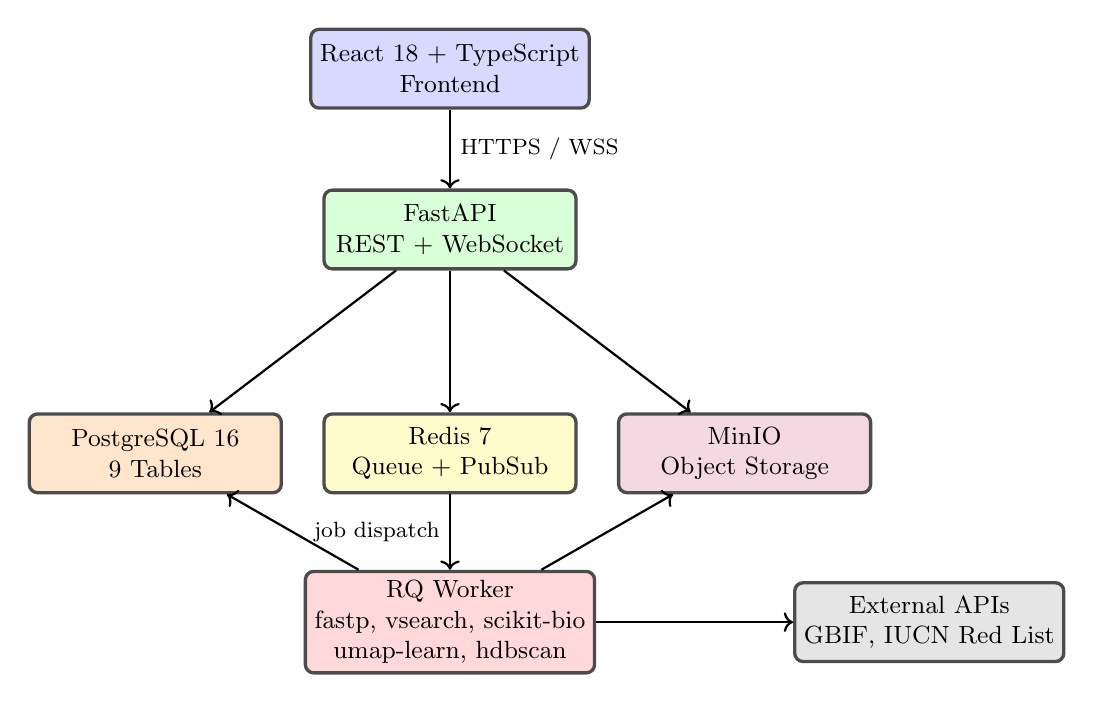
\begin{tikzpicture}[
    font=\small,
    arrow/.style={->, thick},
    box/.style={rectangle, rounded corners=3pt, draw=black!70, align=center, minimum height=1cm, minimum width=3.2cm, very thick},
    group/.style={rectangle, draw, dashed, rounded corners, inner sep=0.4cm}
]
\node[box, fill=blue!15] (fe) {React 18 + TypeScript\\Frontend};
\node[box, fill=green!15, below=1.0cm of fe] (api) {FastAPI\\REST + WebSocket};
\node[box, fill=orange!20, below left=1.8cm and 0.5cm of api] (pg) {PostgreSQL 16\\9 Tables};
\node[box, fill=yellow!20, below=1.8cm of api] (redis) {Redis 7\\Queue + PubSub};
\node[box, fill=purple!15, below right=1.8cm and 0.5cm of api] (minio) {MinIO\\Object Storage};
\node[box, fill=red!15, below=3.8cm of api] (worker) {RQ Worker\\fastp, vsearch, scikit-bio\\umap-learn, hdbscan};
\node[box, fill=gray!20, right=2.5cm of worker] (ext) {External APIs\\GBIF, IUCN Red List};
\draw[arrow] (fe) -- node[right, font=\footnotesize]{HTTPS / WSS} (api);
\draw[arrow] (api) -- (pg);
\draw[arrow] (api) -- (redis);
\draw[arrow] (api) -- (minio);
\draw[arrow] (redis) -- node[left, font=\footnotesize]{job dispatch} (worker);
\draw[arrow] (worker) -- (pg);
\draw[arrow] (worker) -- (minio);
\draw[arrow] (worker) -- (ext);
\end{tikzpicture}
}
\caption{Service topology of the Relict platform. Six containers are orchestrated through Docker Compose. The worker container holds all bioinformatics binaries and communicates with external biodiversity APIs for conservation cross-referencing.}
\label{fig:architecture}
\end{figure}

\subsection{Pipeline Stages}

Each uploaded FASTQ file is processed through seven sequential stages (Fig.~\ref{fig:pipeline}).

\textbf{Stage 1: Quality Control.} The fastp tool (version 0.24.0) performs adapter auto-detection and removal, per-base quality filtering at a threshold of Phred $\geq$ 20, sliding window quality trimming, and minimum length enforcement at 50 base pairs. A machine-readable JSON report is generated recording pre- and post-filtering read counts, Q20/Q30 rates, and GC content.

\textbf{Stage 2: Dereplication.} Identical sequences are collapsed using vsearch \texttt{--fastx\_uniques} (version 2.28.1), with the observed abundance of each unique sequence recorded in the FASTA header as a \texttt{size=N} annotation. Sequences observed fewer than two times are discarded as likely artefacts.

\textbf{Stage 3: ASV Inference.} The UNOISE3 algorithm \cite{edgar2016} implemented in vsearch \texttt{--cluster\_unoise} performs error correction on the dereplicated sequences to produce amplicon sequence variants representing biologically real sequence entities cleaned of PCR and sequencing noise.

\textbf{Stage 4: Taxonomy Assignment.} Each ASV centroid is aligned against a version-pinned reference database using vsearch \texttt{--usearch\_global} with a minimum identity threshold of 80\%. The platform currently supports SILVA 138.1 SSU NR99 \cite{quast2013} (436,680 sequences) for 16S and 18S markers, and MIDORI2 GenBank 269 \cite{leray2022} for COI (1,801,886 sequences) and 12S (193,724 sequences) markers. Taxonomy is parsed from reference FASTA headers at seven standard ranks from kingdom through species.

\textbf{Stage 5: Conservation Cross-Referencing.} For each species-level taxonomy assignment, the pipeline queries the GBIF Species API to resolve the canonical taxon name and retrieve global occurrence counts, then queries the GBIF-mirrored IUCN Red List endpoint to obtain the conservation category (LC, NT, VU, EN, CR, EW, or EX) and population trend where available. Results are cached in PostgreSQL with a 30-day time-to-live to limit external API load. The provenance manifest records the retrieval timestamp for each conservation record.

\textbf{Stage 6: Diversity Metrics.} Alpha diversity indices are computed from the ASV abundance vector using scikit-bio (version 0.6.2): Shannon entropy ($H' = -\sum p_i \ln p_i$), Simpson index ($1 - \sum p_i^2$), Chao1 estimated richness, observed richness, and Pielou's evenness ($J' = H' / \ln S$).

\textbf{Stage 7: Provenance Manifest.} A JSON document is generated recording every input file SHA256, all tool versions, the reference database identity, pipeline parameters as a deterministic hash, per-stage runtimes, and a SHA256 signature computed over the canonical (sorted, compact) JSON representation of the manifest body.

\begin{figure}[t]
\centering
\resizebox{0.65\textwidth}{!}{%
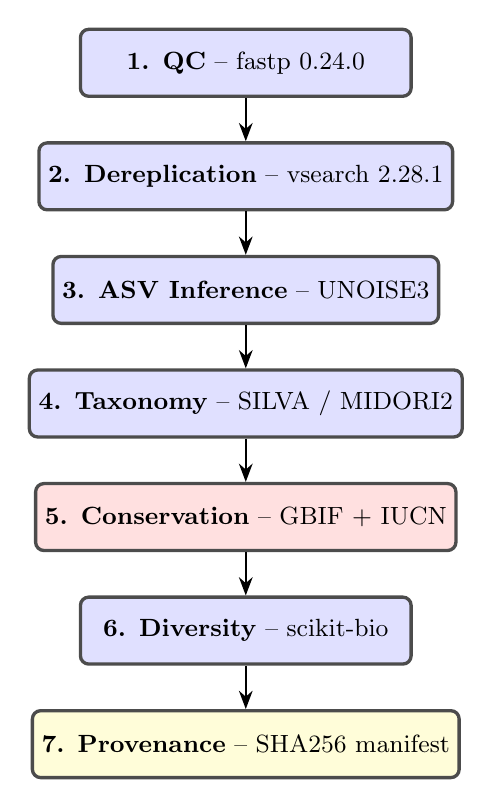
\begin{tikzpicture}[
    font=\small,
    node distance=0.55cm,
    >=Stealth,
    stage/.style={rectangle, rounded corners=3pt, draw=black!70, minimum width=4.2cm, minimum height=0.85cm, align=center, very thick},
    arrow/.style={->, thick}
]
\node[stage, fill=blue!12] (qc) {\textbf{1. QC} -- fastp 0.24.0};
\node[stage, fill=blue!12, below=of qc] (derep) {\textbf{2. Dereplication} -- vsearch 2.28.1};
\node[stage, fill=blue!12, below=of derep] (denoise) {\textbf{3. ASV Inference} -- UNOISE3};
\node[stage, fill=blue!12, below=of denoise] (tax) {\textbf{4. Taxonomy} -- SILVA / MIDORI2};
\node[stage, fill=red!12, below=of tax] (cons) {\textbf{5. Conservation} -- GBIF + IUCN};
\node[stage, fill=blue!12, below=of cons] (div) {\textbf{6. Diversity} -- scikit-bio};
\node[stage, fill=yellow!15, below=of div] (prov) {\textbf{7. Provenance} -- SHA256 manifest};
\draw[arrow] (qc) -- (derep);
\draw[arrow] (derep) -- (denoise);
\draw[arrow] (denoise) -- (tax);
\draw[arrow] (tax) -- (cons);
\draw[arrow] (cons) -- (div);
\draw[arrow] (div) -- (prov);
\end{tikzpicture}
}
\caption{Sequential pipeline stages. Stage 5 (conservation) queries external biodiversity databases for each detected taxon. Stage 7 produces a signed manifest recording all inputs, versions, and outputs.}
\label{fig:pipeline}
\end{figure}

\subsection{Amplicon Marker Support}

The platform ships with YAML-based preset configurations for six amplicon markers (Table~\ref{tab:markers}), each specifying primer sequences, expected amplicon length ranges, quality control parameters, denoising thresholds, taxonomy identity cutoffs, and the recommended reference database.

\begin{table}[t]
\centering
\caption{Supported amplicon markers and preset configurations.}
\label{tab:markers}
\begin{tabular}{llcll}
\toprule
\textbf{Marker} & \textbf{Primers} & \textbf{Length (bp)} & \textbf{Reference DB} & \textbf{Target Organisms} \\
\midrule
16S V4    & 515F / 806R           & 200--350 & SILVA 138.1      & Bacteria, Archaea \\
12S MiFish & MiFish-U-F / -R      & 163--185 & MIDORI2 srRNA    & Fish, vertebrates \\
COI Leray  & mlCOIintF / jgHCO2198 & 280--340 & MIDORI2 CO1     & Invertebrates \\
18S V9    & 1391F / EukBr         & 100--200 & SILVA 138.1      & Eukaryotes \\
rbcL      & rbcLa-F / -R          & 500--600 & SILVA 138.1      & Plants \\
ITS2      & fITS7 / ITS4          & 200--450 & SILVA 138.1      & Fungi \\
\bottomrule
\end{tabular}
\end{table}

\subsection{Output Formats}

Each completed analysis produces five downloadable outputs through the web interface: an interactive dashboard displaying diversity metrics, taxonomy tables with IUCN conservation badges, and provenance details; a Darwin Core Archive conforming to the GBIF DNA-derived data publishing standard \cite{gbif2023}; a flat CSV containing ASV sequences, abundances, taxonomy assignments, and identity scores; a BIOM 2.1.0 JSON file compatible with QIIME~2 and phyloseq \cite{mcmurdie2013}; and the signed provenance manifest in JSON format.

\section{Experimental Evaluation}

\subsection{Synthetic Benchmark}

To verify computational correctness, a controlled dataset was constructed from 100 reads originating from five bacterial species (\textit{Escherichia coli}, \textit{Bacillus subtilis}, \textit{Staphylococcus aureus}, \textit{Pseudomonas aeruginosa}, \textit{Lactobacillus rhamnosus}) at uniform abundance of 20 reads per species. The sequences correspond to real 16S V4 amplicon regions extracted from GenBank accessions. Under these conditions, theoretically exact diversity metrics can be computed: Shannon entropy equals $\ln 5 \approx 1.6094$, Simpson index equals $1 - 1/5 = 0.8$, and Pielou's evenness equals unity.

All ten automated benchmark checks passed (Table~\ref{tab:synthetic}). The pipeline correctly identified five ASVs, assigned taxonomy to all five at genus level against SILVA 138.1, and resolved all five against GBIF.

\begin{table}[t]
\centering
\caption{Synthetic benchmark results. All ten checks passed with expected values.}
\label{tab:synthetic}
\begin{tabular}{llll}
\toprule
\textbf{Metric} & \textbf{Expected} & \textbf{Observed} & \textbf{Result} \\
\midrule
ASV count             & 5                & 5               & Pass \\
Taxonomy assignment   & 5/5 (100\%)      & 5/5             & Pass \\
Known genera detected & $\geq$3 of 4     & 4/4             & Pass \\
Shannon index ($H'$)  & $\ln 5 = 1.6094$ & 1.6094          & Pass \\
Simpson index ($1-D$) & 0.8000           & 0.8000          & Pass \\
Pielou's evenness     & 1.0000           & 1.0000          & Pass \\
Species richness      & 5                & 5               & Pass \\
Chao1 estimate        & 5.0              & 5.0             & Pass \\
GBIF resolution       & $\geq$3/5        & 5/5             & Pass \\
Provenance manifest   & Valid SHA256      & Valid           & Pass \\
\bottomrule
\end{tabular}
\end{table}

\subsection{Published Dataset Benchmark}

The pipeline was further evaluated on ERR2283086, a mock bacterial community dataset publicly available from the European Nucleotide Archive comprising 45,204 Illumina MiSeq paired-end reads at 151 base pairs. Processing completed in 215 seconds across all seven stages (Table~\ref{tab:sra}).

\begin{table}[t]
\centering
\caption{Performance on published SRA dataset ERR2283086 (mock community).}
\label{tab:sra}
\begin{tabular}{ll}
\toprule
\textbf{Metric} & \textbf{Value} \\
\midrule
Input reads              & 45,204 \\
ASVs detected            & 51 \\
Taxonomy assignment rate & 51/51 (100\%) \\
Reference identity       & 100\% (all top hits) \\
Shannon entropy ($H'$)   & 2.585 \\
Simpson index ($1-D$)    & 0.888 \\
Chao1 estimated richness & 51.0 \\
Pielou's evenness ($J'$) & 0.657 \\
Pipeline runtime         & 215 s \\
Phyla recovered          & 3 \\
Dominant genus           & \textit{Acinetobacter} (7,266 reads) \\
\bottomrule
\end{tabular}
\end{table}

The recovered community spanned three bacterial phyla (Proteobacteria, Firmicutes, Actinobacteriota) distributed across fifteen genera with ecologically plausible abundance patterns. All taxonomy assignments achieved 100\% identity against SILVA 138.1 reference sequences. The conservation cross-referencing module resolved all detected species against GBIF, returning IUCN status codes consistent with the bacterial taxa examined (NE, Not Evaluated, which is the correct designation for microbial species not within the scope of IUCN assessments).

\section{Assumptions and Limitations}

The platform inherits the well-characterised biological limitations of eDNA metabarcoding: primer binding bias, differential PCR amplification, reference database gaps, and the inability to distinguish between DNA from living organisms and residual environmental DNA from deceased individuals \cite{taberlet2012}. Relict does not attempt to correct for these effects; it instead makes them transparent through comprehensive provenance documentation.

The conservation cross-referencing component depends on the availability and currency of GBIF and IUCN data services. External API responses are cached locally with a thirty-day retention period, and the provenance manifest records the exact retrieval timestamp for each conservation record to allow users to assess potential staleness.

The current pipeline employs vsearch for ASV inference using the UNOISE3 algorithm. While DADA2 \cite{callahan2016} is generally considered the reference standard for Illumina error modelling, vsearch offers substantially faster processing with comparable output quality and considerably simpler deployment requirements. Integration of DADA2 as an alternative inference path is planned for a subsequent release.

Taxonomy assignment accuracy is bounded by reference database completeness. Species-level identifications for taxa that are poorly represented in SILVA or MIDORI2 should be treated with appropriate caution, particularly for amplicon markers with limited phylogenetic resolution among closely related species.

\section{Software Availability}

Relict is distributed under the MIT licence. The complete source code, deployment configuration, reference database download scripts with SHA256 verification, benchmark datasets, amplicon preset files, and documentation are maintained at \url{https://github.com/ShAuRyA-Noodle/Bad-Omens}. Deployment requires Docker and Docker Compose. A machine-readable citation file (\texttt{CITATION.cff}) is included in the repository root.

\subsection*{Author Contributions}

Shaurya Punj conceived the project, designed the architecture, implemented all system components, conducted the experimental evaluation, and wrote this paper.

\subsection*{Data Availability}

The synthetic benchmark dataset is distributed with the source code. The SRA benchmark dataset ERR2283086 is publicly available from the European Nucleotide Archive at \url{https://www.ebi.ac.uk/ena/browser/view/ERR2283086}. Benchmark results and provenance manifests are archived in the \texttt{docs/benchmarks/} directory of the repository.

\subsection*{ORCID}

Shaurya Punj \quad \url{https://orcid.org/0009-0000-7351-0237}

\bibliographystyle{splncs04}

\begin{thebibliography}{19}

\bibitem{bolyen2019}
Bolyen, E., Rideout, J.R., Dillon, M.R., et al.: Reproducible, interactive, scalable and extensible microbiome data science using QIIME~2. Nature Biotechnology \textbf{37}, 852--857 (2019)

\bibitem{bonfil2021}
Bonfil, R., Palacios-Barreto, P., Vargas, O.U.M., et al.: Detection of critically endangered marine species with dwindling populations using eDNA. Marine Biology \textbf{168}(5), 1--12 (2021)

\bibitem{boyer2016}
Boyer, F., Mercier, C., Bonin, A., et al.: obitools: a unix-inspired software package for DNA metabarcoding. Molecular Ecology Resources \textbf{16}(1), 176--182 (2016)

\bibitem{callahan2016}
Callahan, B.J., McMurdie, P.J., Rosen, M.J., et al.: DADA2: High-resolution sample inference from Illumina amplicon data. Nature Methods \textbf{13}(7), 581--583 (2016)

\bibitem{deiner2017}
Deiner, K., Bik, H.M., M{\"a}chler, E., et al.: Environmental DNA metabarcoding: Transforming how we survey animal and plant communities. Molecular Ecology \textbf{26}(21), 5872--5895 (2017)

\bibitem{edgar2016}
Edgar, R.C.: UNOISE2: improved error-correction for Illumina 16S and ITS amplicon sequencing. bioRxiv, 081257 (2016)

\bibitem{ficetola2008}
Ficetola, G.F., Miaud, C., Pompanon, F., Taberlet, P.: Species detection using environmental DNA from water samples. Biology Letters \textbf{4}(4), 423--425 (2008)

\bibitem{gbif2023}
GBIF Secretariat: Publishing DNA-derived data through biodiversity data platforms. \url{https://docs.gbif.org/publishing-dna-derived-data/en/} (2023)

\bibitem{larson2020}
Larson, E.R., Graham, B.M., Achury, R., et al.: From eDNA to citizen science: Emerging tools for the early detection of invasive species. Frontiers in Ecology and the Environment \textbf{18}(4), 194--202 (2020)

\bibitem{lee2024}
Lee, K.N., Kelly, R.P., Demir-Hilton, E., et al.: Adoption of environmental DNA in public agency practice. Environmental DNA \textbf{6}(1), 1--14 (2024)

\bibitem{leray2022}
Leray, M., Knowlton, N., Machida, R.J.: MIDORI2: A collection of quality-controlled, preformatted, and regularly updated reference databases for taxonomic assignment of eukaryotic mitochondrial sequences. Environmental DNA \textbf{4}(4), 894--907 (2022)

\bibitem{mcmurdie2013}
McMurdie, P.J., Holmes, S.: phyloseq: An R package for reproducible interactive analysis and graphics of microbiome census data. PLoS ONE \textbf{8}(4), e61217 (2013)

\bibitem{pfleger2016}
Pfleger, M.O., Rider, S.J., Johnston, C.E., Janosik, A.M.: Saving the doomed: Using eDNA to aid in detection of rare sturgeon for conservation. Global Ecology and Conservation \textbf{8}, 99--107 (2016)

\bibitem{powers2019}
Powers, S.M., Hampton, S.E.: Open science, reproducibility, and transparency in ecology. Ecological Applications \textbf{29}(1), e01822 (2019)

\bibitem{quast2013}
Quast, C., Pruesse, E., Yilmaz, P., et al.: The SILVA ribosomal RNA gene database project: Improved data processing and web-based tools. Nucleic Acids Research \textbf{41}(D1), D590--D596 (2013)

\bibitem{rognes2016}
Rognes, T., Flouri, T., Nichols, B., Quince, C., Mah{\'e}, F.: VSEARCH: A versatile open source tool for metagenomics. PeerJ \textbf{4}, e2584 (2016)

\bibitem{sandve2013}
Sandve, G.K., Nekrutenko, A., Taylor, J., Hovig, E.: Ten simple rules for reproducible computational research. PLoS Computational Biology \textbf{9}(10), e1003285 (2013)

\bibitem{schloss2011}
Schloss, P.D., Westcott, S.L.: Assessing and improving methods used in operational taxonomic unit-based approaches for 16S rRNA gene sequence analysis. Applied and Environmental Microbiology \textbf{77}, 3219--3226 (2011)

\bibitem{taberlet2012}
Taberlet, P., Coissac, E., Hajibabaei, M., Rieseberg, L.H.: Environmental DNA. Molecular Ecology \textbf{21}(8), 1789--1793 (2012)

\bibitem{williams2024}
Williams, J., Pettorelli, N., Dowell, R., et al.: SimpleMetaPipeline: Breaking the bioinformatics bottleneck in metabarcoding. Methods in Ecology and Evolution \textbf{15}, 1949--1957 (2024)

\end{thebibliography}

\end{document}
